\chapter{Small oscillations}
\section{Potential energy and equilibrium}
In order to understand the general theory of oscillations, it is essential to know about the potential energl at the equilibrium configuration. Let us consider a conservative system in which the potential energy is: function of position only. Let the system be specified by $n$ generalized coordinates $q_{1}, q_{2}, \ldots, q_{n}$, not involve, time explicitly. For such a system, the potential energy is given by
$$
V=V\left(q_{1}, q_{2}, \ldots, q_{n}\right)
$$
and the generalized forces are given by
$G_{k}=-\frac{\partial V}{\partial q_{k}}$ where $k=1,2, \ldots ., n$\\
The system is said to be in equilibrium, if the generalized forces acting on the system are equal to zero: i.e.,
$$
G_{k}=-\left[\frac{\partial V}{\partial q_{k}}\right]_{0}=0
$$
\textbf{For small oscillations}\\
\textbf{Force constant} $k=\left.\frac{\partial^{2} V}{\partial q_k^{2}}\right|_{q=q_{0}} \text { where } q_{0} \text { is stable equilibrium point. }$\\
\textbf{Angular frequency} $\omega=\sqrt{\frac{k}{m}}$
\subsection{Stable,Unstable and Neutral equilibrium}
\subsubsection{Stable equilibrium}
A system is said to be in stable equilibrium, if a small displacement of the system from the rest position (by giving a little energy to it) results in a small bounded motion about the equilibrium position.
\subsubsection{Unstable equilibrium}
Small displacement of the system from the equilibrium position results in an unbounded motion, it is in an unstable equilibrium.
\subsubsection{Neutral equilibrium}
 Further, if the system on displacement has no tendency to move about or away the equilibrium position, it is said to be in neutral equilibrium.\\
 \begin{minipage}{0.5\textwidth}
 \begin{figure}[H]
 	\centering
 	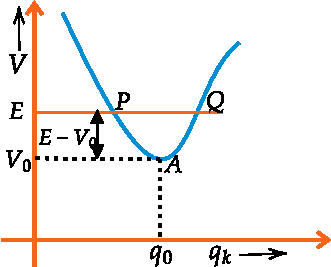
\includegraphics[height=4cm,width=5cm]{stable}
 	\caption{}
 	\label{fig1}
 \end{figure}
 \end{minipage}
\begin{minipage}{0.5\textwidth}
\begin{figure}[H]
	\centering
	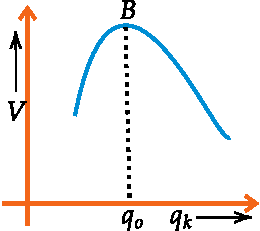
\includegraphics[height=3cm,width=5cm]{unstable}
	\caption{}
	\label{fig2}
\end{figure}
\end{minipage}
A graph drawn between the potential energy of the system and a particular coordinate $q_{k}$ is called potential energy curve and  The positions $A$ and $B$, where the generalized force $F=-\partial V / \partial q$ vanishes, are the positions of equilibrium; potential energy $V$ is minimum (say $V_{0}$ ) at $A$ [fig.\ref{fig1}] and maximum at $B$ [fig.\ref{fig2} ]. Position $A$ corresponds to the stable equilibrium, because if the system is displaced from $A$ to $Q$ by giving energy $\left(E-V_{0}\right)$ and left to itself, the system tries to come in the position of minimum potential energy. Consequently the potential energy will change to kinetic energy and at $A$ the energy $\left(E-V_{0}\right)$ will be purely in the kinetic form because of the conservation law. This will change again to potential form, when the system moves towards the position $P$ and hence a bounded motion ensues about the equilibrium position $A$. Obviously the position $B$ of the maximum potential energy represents the unstable equilibrium because any energy given to the system at this position will result more and more kinetic energy when the system moves either left or right to it. In this case, the system moves away from the equilibrium position. In case of neutral equilibrium, the potential energy is independent of the coordinate and equilibrium. occurs at any arbitrary value of that coordinate.
\section{Small oscillations}
In small oscillation we generalize the harmonic oscillator problem of one degree of freedom in the lagrangian formulation to the case of small amplitude oscillations of a system of seversl degrees of freedom near the position of equilibrium.When we go from a single oscillator to the problem of two coupled oscillators the analysis results in some interesting and surprising new features.We shall see that the motion of the two coupled oscillators in general is much complicated and none of the oscillators in general executes simple harmonic motion.However for small amplitude oscillations ,we may express the general motion as a superposition of two independant simple harmonic motions ,both going on simultaneously.We call thsese two simple harmonic motions as normal modes or simply modes.Further we shall see that a system of N coupled oscillators with N degrees of freedom ,has exactly N independant modes of vibration and general motion can be expressed as the superposition of N normal modes.Each mode has its own frquency and wavelength.
\subsection{Matrix method to solve small oscillations}
We shall interested in the motion of the system with in the immediate neighbourhood of configuration of stable equilibrium .Since the departure fro the equilibrium is very small ,all functions may be expanded in a Taylor series about the equlibrium ,retaining only the lowest order terms .The deviation of the generalized coordinates from equilibrium will be denoted by $\eta_i$:\\
$$q_i=q_{oi}+\eta_i$$
and these may be taken as the new generalized coordinates of the motion  
\begin{figure}[H]
	\centering
	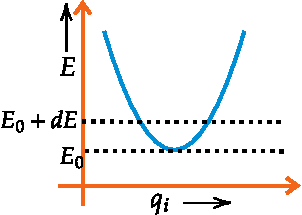
\includegraphics[height=3cm,width=5cm]{potential}
	\caption{}
	\label{}
\end{figure}
One can expand potential energy by Taylor series expansion
$$V\left(q_{i} \ldots \ldots q_{n}\right)=V\left(q_{00} \ldots \ldots q_{0 n}\right)+\left.\frac{\partial V}{\partial q_{i}}\right|_{q_{i 0}}\left(q_{i}-q_{0 i}\right)+\frac{1}{2} \frac{\partial^{2} V}{\partial q_{i} \partial q_{j}}\left(q_{i}-q_{0 i}\right)\left(q_{j}-q_{0 j}\right)+\ldots .$$
The 0 in subscript means $q_{i}=q_{0 i}$\\
So,
\begin{equation}
\quad V(q)=V_{0}+0+\frac{1}{2}\left(\frac{\partial^{2} V}{\partial q_{i} \partial q_{j}}\right)_{0} \eta_{i} \eta_{j}+\ldots \ldots \label{ref1}
\end{equation}
because at equilibrium,
$$
\left(\frac{\partial V}{\partial q_{i}}\right)_{q_{i}=q_{0 i}} \equiv\left(\frac{\partial V}{\partial q_{i}}\right)_{0}=-Q_{i}=0
$$
where $Q_{i}$ is the generalized force. Now,
\begin{equation}
V_{0} \equiv V\left(q_{01}, q_{02}, \ldots \ldots, q_{0 n}\right) \label{ref2}
\end{equation}
 is the potential energy of eqilibrium configuration whis is constant.So we set $V_0$ is equal to zero because in equations of motions only derivative of V occur.\\
 Neglecting higher order terms (because $\eta_{i}^{\prime} s$ are very small)
 \begin{equation}
 V=\frac{1}{2}\left(\frac{\partial^{2} V}{\partial q_{i} \partial q_{j}}\right)_{0} \eta_{i} \eta_{j}=\frac{1}{2} V_{i j} \eta_{i} \eta_{j} \label{ref3}
 \end{equation}
 We see that $V_{i j}=V_{j i}$
 We can write $V$ in matrix form as
\begin{align}
 V=\frac{1}{2}\left(\begin{array}{llll}
\eta_{1} & \eta_{2} & \cdots & \eta_{n}
\end{array}\right)\left[\begin{array}{cccc}
V_{11} & V_{12} & \cdots & V_{1 n} \\
V_{21} & V_{22} & \ldots & V_{2 n} \\
\vdots & \vdots & \ldots & \vdots \\
V_{n 1} & V_{n 2} & \ldots & V_{n n}
\end{array}\right]\left[\begin{array}{l}
\eta_{1} \\
\eta_{2} \\
\vdots \\
\eta_{n}
\end{array}\right]\label{ref4}
\end{align}
Since the constraints are time independent, hence kinetic energy can be written as
\begin{align}
T=\frac{1}{2} m_{i j} \dot{q}_{i} \dot{q}_{j}=\frac{1}{2} m_{i j} \dot{\eta}_{i} \dot{\eta}_{j}\label{ref5}
\end{align}
Since, $q_{i}=q_{0 i}+\eta_{i}$, so $\dot{q}_{i}=\dot{\eta}_{i}$\\
$m_{i j}$ can also be expanded similar to $V$
$$m_{i j}=m_{i j}\left(q_{01}, q_{02}, \ldots \ldots, q_{0 n}\right)+\left(\frac{\partial m_{i j}}{\partial q_{k}}\right)_{0} \dot{\eta}_{k}+\ldots \ldots \ldots$$
$\text { here we take first term only, because in equation $\ref{ref5}$ we already has } \dot{\eta} \dot{\eta}_{j} $.\\
so
\begin{equation}
T=\frac{1}{2} T_{i j} \dot{\eta}_{i} \dot{\eta}_{j}\label{ref6}
\end{equation}
$\text { where, } \quad T_{i j}=m_{i j}\left(q_{01}, q_{02}, \ldots \ldots q_{0 n}\right)$\\
\text { In matrix form, }
\begin{align}
 T=\frac{1}{2}\left(\begin{array}{llll}
\dot{\eta}_{1} & \dot{\eta}_{2} & \ldots & \dot{\eta}_{n}
\end{array}\right)\left[\begin{array}{cccc}
T_{11} & T_{12} & \ldots & T_{1 n} \\
T_{21} & T_{22} & \ldots & T_{2 n} \\
\vdots & \vdots & \ldots & \vdots \\
T_{n 1} & T_{n 2} & \ldots & T_{n n}
\end{array}\right]\left[\begin{array}{l}
\dot{\eta}_{1} \\
\dot{\eta}_{2} \\
\vdots \\
\dot{\eta}_{n}
\end{array}\right]\label{ref7}
\end{align}
Like $\mathbf{V}, \mathbf{T}$ is also symmetric, i.e. $T_{i j}=T_{j i}$
The Lagrangian is, 
\begin{align}
L=T-V=\frac{1}{2}\left(T_{i j} \dot{\eta}_{i} \dot{\eta}_{j}-V_{i j} \eta_{i} \eta_{j}\right)\label{ref8}
\end{align}
The equation of motion for $\eta_{i}$
$$
\frac{d}{d t}\left(\frac{\partial L}{\partial \dot{\eta}_{i}}\right)-\frac{\partial L}{\partial \eta_{i}}=0
$$
\begin{align}
&\frac{d}{d t}\left(\frac{\partial}{\partial \dot{\eta}_{i}}\left(T_{i j} \dot{\eta}_{i} \dot{\eta}_{j}-V_{i j} \eta_{i} \eta_{j}\right)\right)-\frac{\partial}{\partial \eta_{i}}\left(T_{i j} \dot{\eta}_{i} \dot{\eta}_{j}-V_{i j} \eta_{i} \eta_{j}\right)=0 \notag \\
&\frac{d}{d t}\left(T_{i j} \dot{\eta}_{j}\right)-V_{i j} \eta_{j}=0 \notag \\
&T_{i j} \ddot{\eta}_{j}+V_{i j} \eta_{j}=0 \label{ref9}
\end{align}
Note that $T_{i j}$ and $\mathrm{V}_{i j}$ are constants and $\dot{\eta}^{\prime} s$ and $\eta^{\prime} s$ appear only as multiplication with each other. For example the equation for $\eta_{1}$ is
\begin{align*}
&\frac{d}{d t}\left(\frac{\partial L}{\partial \dot{\eta}_{1}}\right)-\frac{\partial L}{\partial \eta_{1}}=0 \\
&\frac{d}{d t}\left[\frac{\partial}{\partial \dot{\eta}_{1}}\left(T_{1 j} \dot{\eta}_{1} \dot{\eta}_{j}\right)+\frac{\partial}{\partial \eta_{1}}\left(V_{1 j} \eta_{1} \eta_{j}\right)\right]=0
\end{align*}
[Since $V$ is independent of $\dot{\eta}^{\prime} s$ and $T$ is independent of $\eta^{\prime} s$ ]. So,
\begin{align*}
&\frac{d}{d t}\left(\frac{\partial}{\partial \dot{\eta}_{1}}\left(T_{11} \dot{\eta}_{1} \dot{\eta}_{1}+T_{12} \dot{\eta}_{1} \dot{\eta}_{2}+\ldots \ldots \ldots .+T_{1 n} \dot{\eta}_{1} \dot{\eta}_{n}+\ldots \ldots . .\right)\right)\\
&+\frac{\partial}{\partial \eta_{1}}\left(V_{11} \eta_{1} \eta_{1}+V_{12} \eta_{1} \eta_{2}+\ldots \ldots . . V_{1 n} \eta_{1} \eta_{n}+\ldots \ldots\right)=0 \\
&\frac{d}{d t}\left(T_{11} \dot{\eta}_{1}+T_{12} \dot{\eta}_{2}+\ldots \ldots T_{1 n} \dot{\eta}_{n}\right)+\left(V_{11} \eta_{1}+V_{12} \eta_{2}+\ldots \ldots+V_{1 n} \eta_{n}\right)=0 \\
&T_{11} \ddot{\eta}_{1}+T_{12} \ddot{\eta}_{2}+\ldots . .+T_{1 n} \ddot{\eta}_{n}+\left(V_{11} \eta_{1}+V_{12} \eta_{2}+\ldots . .+V_{1 n} \eta_{n}\right)=0
\end{align*}
In summation convention the above equation is
\begin{align}
T_{1 j} \ddot{\eta}_{j}+V_{1 j} \eta_{j}=0\label{ref10}
\end{align}
The point is that you should know what any expression means. So, we get $\eta$ equations in total.
To sovle the equation of motion $\eta$, we put a trial solution.

\begin{equation}
\eta_{j}=C a_{j} e^{-i o t}\label{ref11}
\end{equation}
Note that in the exponential $i=\sqrt{-1}$
We get,
\begin{align}
&\dot{\eta}_{j}=-C a_{j}(i \omega) e^{-i \omega t} \notag \\
&\ddot{\eta}_{j}=+C a_{j}(i \omega)^{2} e^{-i \omega t}=-\omega^{2} \eta_{j}\label{ref12}
\end{align}
$\text { putting } \ddot{\eta}_{j} \text { in equation ($\ref{ref9}$) }$
\begin{align}
&T_{i j} \ddot{\eta}_{j}+V_{i j} \eta_{j}=0 \notag\\
&T_{i j}\left(-\omega^{2} \eta_{j}\right)+V_{i j} \eta_{j}=0 \notag\\
&\left(V_{i j}-\omega^{2} T_{i j}\right) \eta_{j}=0\label{ref13} \\
&V_{i j} a_{j}=\omega^{2} T_{i j} a_{j}\label{ref14}
\end{align}
 in the matrix form equation ($\ref{ref13}$), is (equation  $\ref{ref14}$  also can be written in similar form)\\
 $\left[\begin{array}{cccc}
 	V_{11} & V_{12} & \ldots & V_{1 n} \\
 	V_{21} & V_{22} & \ldots & V_{2 n} \\
 	\vdots & \vdots & & \vdots \\
 	V_{n 1} & V_{n 2} & \ldots & V_{n n}
 \end{array}\right]\left[\begin{array}{l}
 	\eta_{1} \\
 	\eta_{2} \\
 	\vdots \\
 	\eta_{n}
 \end{array}\right]-\omega^{2}\left[\begin{array}{cccc}
 	T_{11} & T_{12} & \ldots & T_{1 n} \\
 	T_{21} & T_{22} & \ldots & T_{2 n} \\
 	\vdots & \vdots & & \vdots \\
 	T_{n 1} & T_{n 2} & \ldots & T_{n n}
 \end{array}\right]\left[\begin{array}{l}
 	\eta_{1} \\
 	\eta_{2} \\
 	\vdots \\
 	\eta_{n}
 \end{array}\right]=0$
 \begin{align}
 \left[\begin{array}{cccc}
 V_{11}-\omega^{2} T_{11} & V_{12}-\omega^{2} T_{12} & \ldots & V_{1 n}-\omega^{2} T_{1 n} \\
 V_{21}-\omega^{2} T_{21} & V_{22}-\omega_{2} T_{22} & \ldots & V_{2 n}-\omega^{2} T_{2 n} \\
 \vdots & \vdots & & \vdots \\
 V_{n 1}-\omega^{2} T_{n 1} & V_{n 2}-\omega^{2} T_{n 2} & & V_{n n}-\omega^{2} T_{n n}
 \end{array}\right]\left[\begin{array}{l}
 \eta_{1} \\
 \eta_{2} \\
 \vdots \\
 \eta_{n}
 \end{array}\right]=0\label{ref15}
 \end{align}
 From properties of matrices we know that for equation ($\ref{ref15}$) to be satisfied for all $\eta^{\prime} s$. The determinant of matrix $\mathbf{V}-\omega^{2} \mathbf{T}$ must be zero i.e.
 $$
 \left|\mathbf{V}-\omega^{2} \mathbf{T}\right|=0
 $$
 \begin{align}
 \left|\begin{array}{cccc}
 V_{11}-\omega^{2} T_{11} & V_{12}-\omega^{2} T_{12} & \cdots & V_{1 n}-\omega^{2} T_{1 n} \\
 V_{21}-\omega^{2} T_{21} & V_{22}-\omega_{2} T_{22} & \cdots & V_{2 n}-\omega^{2} T_{2 n} \\
 \vdots & \vdots & & \vdots \\
 V_{n 1}-\omega^{2} T_{n 1} & V_{n 2}-\omega^{2} T_{n 2} & & V_{n n}-\omega^{2} T_{n n}
 \end{array}\right|=0\label{ref16}
 \end{align}
  This equation ($\ref*{ref16}$) is called the secular equation.
  By solving the determinant ($\ref{ref16}$) we get $n$ values of $\omega^{2}$. Each value of $\omega$ represents the frequency of normal mode. The equation ($\ref{ref14}$) is a type of eigenvalues. $\mathbf{V}$ acting on eigenvector a gives $\omega^{2} \mathbf{T a}$. There are $n$ such eigenvectors. Hence, there are $n$ normal modes. It can be shown that the eigen vector matrix of which is denoted by $\mathbf{A}$ diagonalizes both $\mathbf{T}$ and $\mathbf{V}$ (for detail see section $6.2$ of Goldstein, $3^{\text {rd }}$ eddition, but it is sufficient for us to rememher the result). A diagonalizes $\mathbf{V}$ to a matrix whose diagonal elements are the eigen-$\text { values i.e. } \omega^{2 \prime} s \text { (say } \lambda^{\prime} s)$\\
  (Note that in ordinary eigen alue problems, matrix acting on eigenvector produces eigenvalue times the eigenvector i.e. $\mathbf{M a}=\lambda \mathbf{a}$ or $(\mathbf{M}-\lambda \mathbf{1}) \mathbf{a}=0$, but here it is $(\mathbf{V}-\lambda \mathbf{T}) \mathbf{a}=0 .)$\\
  ie
  \begin{align}
  \tilde{\mathbf{A}} \mathbf{V} \mathbf{A}=\lambda=\left[\begin{array}{cccc}
  \lambda_{1} & 0 & \cdots & 0 \\
  0 & \lambda_{2} & \cdots & 0 \\
  \vdots & \vdots & & \vdots \\
  0 & 1, & \cdots & \lambda_{n}
  \end{array}\right]\label{ref17}
  \end{align}
  $\text { where } \lambda_{1}, \lambda_{2} \ldots . . \text { are eigen values of (i.e. } \omega^{21} s \text { ) }$\\
  And $\mathbf{T}$ is diagonalized to identity i.e.
  \begin{align}
  \tilde{\mathbf{A}} \mathbf{T} \mathbf{A}=\mathbf{1}\label{ref18}
  \end{align}
  To solve a problem, the main thing we need to do is\\
   (1) Solve the determinant (9.16) to find the frequencies of normal modes\\
  (2) Find the eigenvectors a correspoinding to each $\omega^{2}$ (the eigenvalue), in the equation.
  $$
  \left(\mathbf{V}-\omega^{2} \mathbf{T}\right) \mathbf{a}=0
  $$
  where the $k^{\text {th }}$ eigenvector (corrersponding to $k^{\text {th }} \omega^{2}$ )
  
  \begin{align}
  \mathbf{a}_{k}=\left[\begin{array}{c}
  a_{1 k} \\
  a_{2 k} \\
  \vdots \\
  a_{n k}
  \end{array}\right]\label{ref19}
  \end{align}
  (3) The normal mode coordinates are
  \begin{align}
  Q_{k}=f_{k} \cos \left(\omega_{k} t+\delta_{k}\right)\label{ref20}
  \end{align}
  where, $f_{k}$ and $\delta_{k}$ are amplitude and phase factor respectively. Note that in a normal mode, the hole system oscillates with same frequency.
  (4) The general solution for
  \begin{align}
  \eta_{i}=a_{i k} Q_{k}\label{ref21}
  \end{align}
   The matrix $\mathbf{A}$ is 
   \begin{align}
   \left[\begin{array}{llll}a_{11} & a_{12} & \cdots & a_{1 n} \\ a_{21} & a_{22} & \cdots & a_{2 n} \\ \vdots & \vdots & & \vdots \\ a_{n 1} & a_{n 2} & \cdots & a_{n n}\end{array}\right]\label{22}
   \end{align}
  So, the solution of our problem (the equation ($\ref{ref21}$) is:
 \begin{align}
  \left[\begin{array}{l}
 \eta_{1} \\
 \eta_{2} \\
 \vdots \\
 \eta_{n}
 \end{array}\right]=\left[\begin{array}{llll}
 a_{11} & a_{12} & \cdots & a_{1 n} \\
 a_{21} & a_{22} & \cdots & a_{2 n} \\
 \vdots & \vdots & & \vdots \\
 a_{n 1} & a_{n 2} & \cdots & a_{n n}
 \end{array}\right]\left[\begin{array}{l}
 Q_{1} \\
 Q_{2} \\
 \vdots \\
 Q_{n}
 \end{array}\right] 
 \end{align}
 One complication may arise when eigenvalues are degenerate. In this case we first choose an eigenvector (corresponding to degenerate eigenvalue) satisfying the eigenvalue equation and remaining eigenvectors (if there is $k$-fold degeneracy, then there are $k$-eigenvectors corresponding to single eigenvalue) are determined such that they satisfy the eigenvalue equation and are orthogonal to each other.
 \newpage
 \begin{abox}
 	Practice set 1
 	\end{abox}
 \begin{enumerate}
 		\item  A particle of unit mass moves in a potential $V(x)=a x^{2}+\frac{b}{x^{2}}$, where $a$ and $b$ are positive constants. The angular frequency of small oscillations about the minimum of the potential is
 		{\exyear{NET JUNE 2011}}
 	\begin{tasks}(2)
 		\task[\textbf{A.}] $\sqrt{8 b}$
 		\task[\textbf{B.}]$\sqrt{8 a}$
 		\task[\textbf{C.}] $\sqrt{8 a / b}$
 		\task[\textbf{D.}]$\sqrt{8 b / a}$
 	\end{tasks}
 	\item Consider the motion of a classical particle in a one dimensional double-well potential $V(x)=\frac{1}{4}\left(x^{2}-2\right)^{2} .$ If the particle is displaced infinitesimally from the minimum on the $x$-axis (and friction is neglected), then
 	{\exyear{NET JUNE 2012}}
 \begin{tasks}(1)
 	\task[\textbf{A.}] the particle will execute simple harmonic motion in the right well with an angular frequency $\omega=\sqrt{2}$
 	\task[\textbf{B.}]the particle will execute simple harmonic motion in the right well with an angular frequency $\omega=2$
 	\task[\textbf{C.}]the particle will switch between the right and left wells
 	\task[\textbf{D.}]the particle will approach the bottom of the right well and settle there
 \end{tasks}
	\item Three particles of equal mass $(\mathrm{m})$ are connected by two identical massless springs of stiffness constant $(K)$ as shown in the figure\\
	\begin{figure}[H]
		\centering
		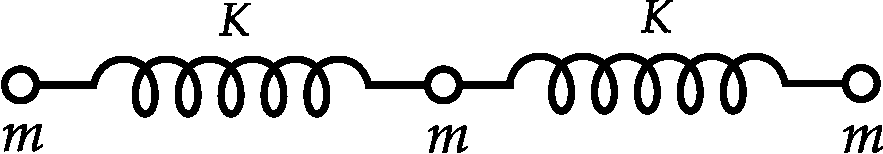
\includegraphics[height=1cm,width=5cm]{problem1}
	\end{figure}
	If $x_{1}, x_{2}$ and $x_{3}$ denote the horizontal displacement of the masses from their respective equilibrium positions the potential energy of the system is
	{\exyear{NET DEC 2012}}
\begin{tasks}(2)
	\task[\textbf{A.}] $\frac{1}{2} K\left[x_{1}^{2}+x_{2}^{2}+x_{3}^{2}\right]$
	\task[\textbf{B.}]$\frac{1}{2} K\left[x_{1}^{2}+x_{2}^{2}+x_{3}^{2}-x_{2}\left(x_{1}+x_{3}\right)\right]$
	\task[\textbf{C.}]$\frac{1}{2} K\left[x_{1}^{2}+2 x_{2}^{2}+x_{3}^{2}-2 x_{2}\left(x_{1}+x_{3}\right)\right]$
	\task[\textbf{D.}]$\frac{1}{2} K\left[x_{1}^{2}+2 x_{2}^{2}-2 x_{2}\left(x_{1}+x_{3}\right)\right]$
\end{tasks}
	\item The time period of a simple pendulum under the influence of the acceleration due to gravity $g$ is $T$. The bob is subjected to an additional acceleration of magnitude $\sqrt{3} g$ in the horizontal direction. Assuming small oscillations, the mean position and time period of oscillation, respectively, of the bob will be
	{\exyear{NET JUNE 2014}}
\begin{tasks}(2)
	\task[\textbf{A.}] $0^{\circ}$ to the vertical and $\sqrt{3} T$
	\task[\textbf{B.}]$30^{\circ}$ to the vertical and $T / 2$
	\task[\textbf{C.}]$60^{\circ}$ to the vertical and $T / \sqrt{2}$
	\task[\textbf{D.}]$0^{\circ}$ to the vertical and $T / \sqrt{3}$
\end{tasks}
	\item A particle of mass $m$ is moving in the potential $V(x)=-\frac{1}{2} a x^{2}+\frac{1}{4} b x^{4}$ where $a, b$ are positive constants. The frequency of small oscillations about a point of stable equilibrium is
	{\exyear{NET DEC 2014}}
\begin{tasks}(2)
	\task[\textbf{A.}] $\sqrt{a / m}$
	\task[\textbf{B.}]$\sqrt{2 a / m}$
	\task[\textbf{C.}]$\sqrt{3 a / m}$
	\task[\textbf{D.}]$\sqrt{6 a / m}$
\end{tasks}
	\item A particle of mass $m$, kept in potential $V(x)=-\frac{1}{2} k x^{2}+\frac{1}{4} \lambda x^{4}$ (where $k$ and $\lambda$ are positive constants), undergoes small oscillations about an equilibrium point. The frequency of oscillations is
	{\exyear{NET JUNE 2018}}
\begin{tasks}(2)
	\task[\textbf{A.}] $\frac{1}{2 \pi} \sqrt{\frac{2 \lambda}{m}}$
	\task[\textbf{B.}]$\frac{1}{2 \pi} \sqrt{\frac{k}{m}}$
	\task[\textbf{C.}]$\frac{1}{2 \pi} \sqrt{\frac{2 k}{m}}$
	\task[\textbf{D.}]$\frac{1}{2 \pi} \sqrt{\frac{\lambda}{m}}$
\end{tasks}
 \end{enumerate}
\colorlet{ocre1}{ocre!70!}
\colorlet{ocrel}{ocre!30!}
\setlength\arrayrulewidth{1pt}
\begin{table}[H]
	\centering
	\arrayrulecolor{ocre}
	
	\begin{tabular}{|p{1.5cm}|p{1.5cm}||p{1.5cm}|p{1.5cm}|}
		\hline
		\multicolumn{4}{|c|}{\textbf{Answer key}}\\\hline\hline
		\rowcolor{ocrel}Q.No.&Answer&Q.No.&Answer\\\hline
		1&\textbf{b}&2&\textbf{b}\\\hline
		3&\textbf{c}&4&\textbf{c}\\\hline
		5&\textbf{b}&6&\textbf{c}\\\hline
	\end{tabular}
\end{table}
\newpage
\begin{abox}
	Practice set 2 
	\end{abox}
\begin{enumerate}

	\item A particle is placed in a region with the potential $V(x)=\frac{1}{2} k x^{2}-\frac{\lambda}{3} x^{3}$, where $k, \lambda>0$.
	Then,
	{\exyear{GATE 2010}}
\begin{tasks}(1)
	\task[\textbf{A.}] $x=0$ and $x=\frac{k}{\lambda}$ are points of stable equilibrium
	\task[\textbf{B.}]$x=0$ is a point of stable equilibrium and $x=\frac{k}{\lambda}$ is a point of unstable equilibrium
	\task[\textbf{C.}]$x=0$ and $x=\frac{k}{\lambda}$ are points of unstable equilibrium
	\task[\textbf{D.}]There are no points of stable or unstable equilibrium
\end{tasks}

	\item Two bodies of mass $m$ and $2 m$ are connected by a spring constant $k$. The frequency of the normal mode is
	{\exyear{GATE 2011}}
\begin{tasks}(2)
	\task[\textbf{A.}] $\sqrt{3 k / 2 m}$
	\task[\textbf{B.}]$\sqrt{k / m}$
	\task[\textbf{C.}] $\sqrt{2 k / 3 m}$
	\task[\textbf{D.}]$\sqrt{k / 2 m}$
\end{tasks}
	\item A particle of unit mass moves along the $x$-axis under the influence of a potential, $V(x)=x(x-2)^{2}$. The particle is found to be in stable equilibrium at the point $x=2$. The time period of oscillation of the particle is
	{\exyear{GATE 2012}}
\begin{tasks}(2)
	\task[\textbf{A.}] $\frac{\pi}{2}$
	\task[\textbf{B.}]$\pi$
	\task[\textbf{C.}]$\frac{3 \pi}{2}$
	\task[\textbf{D.}]$2 \pi$
\end{tasks}

	\item Consider two small blocks, each of mass $M$, attached to two identical springs. One of the springs is attached to the wall, as shown in the figure. The spring constant of each spring is $k$. The masses slide along the surface and the friction is negligible. The frequency of one of the normal modes of the system is,
{	\exyear{GATE 2013}}
	\begin{figure}[H]
		\centering
		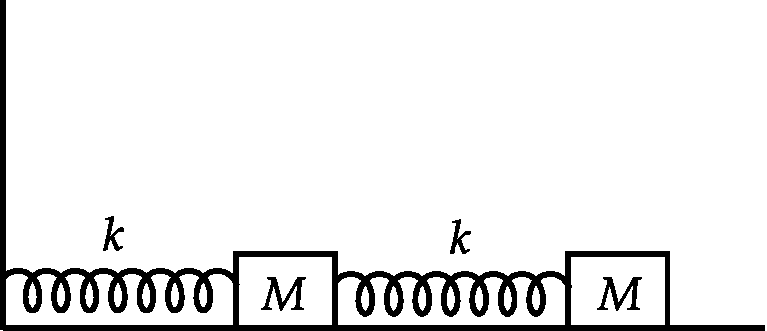
\includegraphics[height=3cm,width=5cm]{GATE1}
	\end{figure}
\begin{tasks}(2)
	\task[\textbf{A.}] $\sqrt{\frac{3+\sqrt{2}}{2}} \sqrt{\frac{k}{M}}$
	\task[\textbf{B.}]$\sqrt{\frac{3+\sqrt{3}}{2} \sqrt{\frac{k}{M}}}$
	\task[\textbf{C.}]$\sqrt{\frac{3+\sqrt{5}}{2}} \sqrt{\frac{k}{M}}$
	\task[\textbf{D.}]$\sqrt{\frac{3+\sqrt{6}}{2}} \sqrt{\frac{k}{M}}$
\end{tasks}

	\item Two masses $m$ and $3 m$ are attached to the two ends of a massless spring with force constant $K$. If $m=100 \mathrm{~g}$ and $K=0.3 \mathrm{~N} / \mathrm{m}$, then the natural angular frequency of oscillation is $H z$.
{	\exyear{GATE 2014}}

	\item A particle of mass $m$ is in a potential given by
	$$
	V(r)=-\frac{a}{r}+\frac{a r_{0}^{2}}{3 r^{3}}
	$$
	where $a$ and $r_{0}$ are positive constants. When disturbed slightly from its stable equilibrium position it undergoes a simple harmonic oscillation. The time period of oscillation is
	{\exyear{GATE 2014}}
\begin{tasks}(2)
	\task[\textbf{A.}] $2 \pi \sqrt{\frac{m r_{0}^{3}}{2 a}}$
	\task[\textbf{B.}]$2 \pi \sqrt{\frac{m r_{0}{ }^{3}}{a}}$
	\task[\textbf{C.}]$2 \pi \sqrt{\frac{2 m r_{0}^{3}}{a}}$
	\task[\textbf{D.}]$4 \pi \sqrt{\frac{m r_{0}^{3}}{a}}$
\end{tasks}

	\item Two identical masses of $10 \mathrm{gm}$ each are connected by a massless spring of spring constant $1 \mathrm{~N} / \mathrm{m}$. The non-zero angular eigenfrequency of the system is. $. \mathrm{rad} / \mathrm{s} .$ (up to two decimal places)
{	\exyear{GATE 2017}}
	\item In the context of small oscillations, which one of the following does NOT apply to the normal coordinates?
	{\exyear{GATE 2018}}
\begin{tasks}(1)
	\task[\textbf{A.}] Each normal coordinate has an eigen-frequency associated with it
	\task[\textbf{B.}]The normal coordinates are orthogonal to one another
	\task[\textbf{C.}]The normal coordinates are all independent
	\task[\textbf{D.}]The potential energy of the system is a sum of squares of the normal coordinates with constant coefficients
\end{tasks}
\end{enumerate}
\colorlet{ocre1}{ocre!70!}
\colorlet{ocrel}{ocre!30!}
\setlength\arrayrulewidth{1pt}
\begin{table}[H]
	\centering
	\arrayrulecolor{ocre}
	
	\begin{tabular}{|p{1.5cm}|p{1.5cm}||p{1.5cm}|p{1.5cm}|}
		\hline
		\multicolumn{4}{|c|}{\textbf{Answer key}}\\\hline\hline
		\rowcolor{ocrel}Q.No.&Answer&Q.No.&Answer\\\hline
		1&\textbf{b}&2&\textbf{a}\\\hline
		3&\textbf{b}&4&\textbf{c}\\\hline
		5&\textbf{0.318}&6&\textbf{a}\\\hline
		7&\textbf{14.14}&8&\textbf{b}\\\hline
	\end{tabular}
\end{table}
\newpage
\begin{abox}
	Practice set 3 
	\end{abox}
\begin{enumerate}
		\item  A particle of mass $m$ moves in one dimension under the influence of a potential energy
	$$
	V(x)=-a\left(\frac{x}{\ell}\right)^{2}+b\left(\frac{x}{\ell}\right)^{4}
	$$
	where $a$ and $b$ are positive constants and $\ell$ is a characteristic length. The frequency of small oscillations about a point of stable equilibrium is:
	\begin{tasks}(2)
		\task[\textbf{a.}] $\frac{1}{2 \pi \ell} \sqrt{\frac{b}{m}}$
		\task[\textbf{b.}]$\frac{2 b}{\pi \ell} \sqrt{\frac{1}{m a}}$
		\task[\textbf{c.}]$\frac{1}{\pi \ell} \sqrt{\frac{a^{2}}{m b}}$
		\task[\textbf{d.}] $\frac{1}{\pi \ell} \sqrt{\frac{a}{m}}$
	\end{tasks}
	\begin{answer}
		\begin{align*}
		\text{	We have,}
		V(x)&=-a\left(\frac{x}{\ell}\right)^{2}+b\left(\frac{x}{\ell}\right)^{4}
		\intertext{Here first we need to find the stable equilibrium. At equilibrium}
		\frac{\partial V(x)}{\partial x}&=0 \quad \Rightarrow \frac{-2 a x}{\ell^{2}}+\frac{4 b x^{3}}{\ell^{4}}=0 \quad \Rightarrow x\left(\frac{2 b x^{2}}{\ell^{2}}-a\right)=0\\
		\Rightarrow \quad x&=0, x=\pm \ell \sqrt{\frac{a}{2 b}}\\
		\text{Now, }\quad \frac{\partial^{2} V}{\partial x^{2}}&=\frac{-2 a}{\ell^{2}}+\frac{12 b x^{2}}{\ell^{4}}\\
		\text{We see that for }x&=0, \frac{\partial^{2} V}{\partial x^{2}}<0
		\text{hence, here there is unstable equilibrium}\\
		\text{For}\qquad x&=\pm \ell \sqrt{\frac{a}{2 b}},\left(\frac{\partial^{2} V}{\partial x^{2}}\right)_{x=\pm \ell \sqrt{\frac{a}{2 b}}}=-\frac{2 a}{\ell^{2}}+\frac{12 b}{\ell^{4}} \ell^{2} \times \frac{a}{2 b}=\frac{4 a}{\ell^{2}}>0
		\intertext{hence, $x=\pm \ell \sqrt{\frac{a}{2 b}}$ corresponds to stable equilibrium.. Now to find the frequeny, we see that the problemis one dimensional, so matrices $\mathbf{V}$ and $\mathbf{T}$ both have one element each, i.e. $V_{11}$ and $T_{11}$ respectively.}
		V_{11}&=\left(\frac{\partial^{2} V}{\partial x^{2}}\right)_{x=\pm f \sqrt{\frac{a}{2 b}}}=\frac{4 a}{\ell^{2}}\\
		\text{Now, the kinetic energy }&=\frac{1}{2} m \dot{x}^{2},\text{ so }T_{11}=m\\
		\text{	Now, we have, }V_{11}-\omega^{2} T_{11}&=0 \qquad\Rightarrow \omega^{2}=\frac{V_{11}}{T_{11}}=\frac{4 a}{m \ell^{2}} \qquad\Rightarrow \omega=\frac{2}{\ell} \sqrt{\frac{a}{m}}\\
		\text{So, the frequency }v&=\frac{\omega}{2 \pi}=\frac{1}{\pi \ell} \sqrt{\frac{a}{m}}
		\intertext{Note: As we have seen in this problem, first we should find the equilibrium configuration of the system then expand potential energy about this configuration in Taylor series.}
		\end{align*}
	\end{answer}
	\item  A particle of mass $m$ is moving in a potential of the form $V(x, y, z)=\frac{1}{2} m \omega^{2}\left(3 x^{2}+3 y^{2}+2 z^{2}+2 x\right)$. The oscillation frequencies of the three normal modes of the particles are given by
\begin{answer}
	\begin{align*}
	\text{The potential is, }V(x, y, z)&=\frac{1}{2} m \omega^{2}\left(3 x^{2}+3 y^{2}+2 z^{2}+2 x y\right)\\
	\text{	Now, }\quad \frac{\partial V}{\partial x}&=0 \quad \Rightarrow 6 x+2 y=0 \quad \Rightarrow y=-3 x\\
	\frac{\partial V}{\partial y}&=0 \quad \Rightarrow 6 y+2 x=0 \quad \Rightarrow y=\frac{-x}{3}\\
	\frac{\partial V}{\partial z}&=0 \quad \Rightarrow z=0\\
	\text{Now, }\quad \frac{\partial^{2} V}{\partial x^{2}}&=3 m \omega^{2}>0 \text{for all $x$}\\
	\frac{\partial^{2} V}{\partial y^{2}}&=3 m \omega^{2}>0\text{ for all $y$}\\
	\text{and }\frac{\partial^{2} V}{\partial z^{2}}&=4>0\text{ for all $z$}
	\intertext{All these conditions tell us that equilibrium point is $(0,0,0)$, because $y=-3 x=-\frac{x}{3}$ satisfies only $x=y=0$ So, the given potential is in the form of expansion about $(0,0,0)$ and the matrix $V_{i j}$ can be written just by inspection.}
	V &=\frac{1}{2} m \omega^{2}\left(3 x^{2}+3 y^{2}+2 z^{2}+2 x y\right) \\ &=\frac{1}{2} m \omega^{2}\left[\begin{array}{lll}x & y & z\end{array}\right]\left[\begin{array}{lll}3 & 1 & 0 \\ 1 & 3 & 0 \\ 0 & 0 & 2\end{array}\right]\left[\begin{array}{l}x \\ y \\ z\end{array}\right]\\
	\text{		because}\quad
	&V=\frac{1}{2}\left(3 m \omega^{2} x^{2}+3 m \omega^{2} y^{2}+2 m \omega^{2} z^{2}+m \omega^{2} x y+m \omega^{2} y x\right) \\
	\text{or,}\quad&V=\frac{1}{2}\left(V_{11} x^{2}+V_{22} y^{2}+V_{33} z^{2}+V_{12} x y+V_{21} y x\right)\\
	\text{	Kinetic energy }T&=\frac{1}{2} m\left(\dot{x}^{2}+\dot{y}^{2}+\dot{z}^{2}\right)=\frac{1}{2}\left[\begin{array}{lll}\dot{x} & \dot{y} & \dot{z}\end{array}\right]\left[\begin{array}{lll}m & 0 & 0 \\ 0 & m & 0 \\ 0 & 0 & m\end{array}\right]\left[\begin{array}{l}\dot{x} \\ \dot{y} \\ \dot{z}\end{array}\right]\\
	\text{Now,}
	\left|\mathbf{V}-\Omega^{2} \mathbf{T}\right|&=0\quad \text{where $\Omega$ is normal mode freuency.}\\
	\Rightarrow \quad&\left|\begin{array}{ccc}3 m \omega^{2}-\Omega^{2} m & m \omega^{2} & 0 \\ m \omega^{2} & 3 m \omega^{2}-\Omega^{2} m & 0 \\ 0 & 0 & 2 m \omega^{2}-\Omega^{2} m\end{array}\right|=0\\
	\Rightarrow \quad\left(2 \omega^{2}-\Omega^{2}\right)&\left[\left(3 \omega^{2}-\Omega^{2}\right)^{2}-\omega^{4}\right]=0 \quad \Rightarrow \Omega_{1}^{2}=2 \omega^{2}\\
	\text{	and }\quad \Omega^{2}&=3 \omega^{2} \pm \omega^{2} \quad \Rightarrow \Omega_{2}^{2}=2 \omega^{2}\text{ and }\Omega_{3}^{2}=4 \omega^{2}
	\intertext{So, the frequencies are $\omega \sqrt{2}, \omega \sqrt{2}$ and $2 \omega$}
	\intertext{	Note that frequencies are always positive, hence we shouldn't write $\Omega_{1}=\pm \omega \sqrt{2}$ etc.}
	\end{align*}
\end{answer}
\item  The Lagrangian of a system is given by $L=\frac{1}{2} m \dot{q}_{1}^{2}+2 m \dot{q}_{2}^{2}-k\left(\frac{5}{4} q_{1}^{2}+2 q_{2}^{2}-2 q_{1} q_{2}\right)$ where $m$ and $k$ are positive constants. The frequencies of its normal modes are
\begin{tasks}(2)
	\task[\textbf{a.}]$\sqrt{\frac{k}{2 m}}, \sqrt{\frac{3 k}{m}}$
	\task[\textbf{b.}]$\sqrt{\frac{k}{2 m}}(13 \pm \sqrt{73})$
	\task[\textbf{c.}]$\sqrt{\frac{5 k}{2 m}}, \sqrt{\frac{k}{m}}$
	\task[\textbf{d.}]  $\sqrt{\frac{k}{2 m}}, \sqrt{\frac{6 k}{m}}$
\end{tasks}
\begin{answer}
	\begin{align*}
	L &=\frac{1}{2} m \dot{q}_{1}^{2}+2 m \dot{q}_{2}^{2}-k\left(\frac{5}{4} q_{1}^{2}+2 q_{2}^{2}-2 q_{1} q_{2}\right) \\ &=\frac{1}{2} m \dot{q}_{1}^{2}+\frac{1}{2} 4 m \dot{q}_{2}^{2}-\frac{1}{2} k\left(\frac{5}{2} q_{1}^{2}+4 q_{2}^{2}-4 q_{1} q_{2}\right) \\ \hat{T} &=\left(\begin{array}{cc}m & 0 \\ 0 & 4 m\end{array}\right), \hat{V}=\left(\begin{array}{cc}\frac{5}{2} k & -2 k \\ -2 k & 4 k\end{array}\right) 
	\intertext{For frequencies of normal modes:}
	\operatorname{det}\left|\omega^{2} \hat{T}-\hat{V}\right|&=0\\
	\left|\begin{array}{cc}\left(m \omega^{2}-\frac{5}{2} k\right) & 2 k \\ 2 k & \left(4 m \omega^{2}-4 k\right)\end{array}\right|&=0 \Rightarrow 4\left(m \omega^{2}-k\right) \frac{\left(2 m \omega^{2}-5 k\right)}{2}-4 k^{2}=0\\
	\Rightarrow 2 m^{2} \omega^{4}+5 k^{2}-7 k m \omega^{2}-2 k^{2}&=0\\
	\Rightarrow 2\left(m \omega^{2}\right)^{2}-7 k\left(m \omega^{2}\right)+3 k^{2}&=0\\
	\Rightarrow m \omega^{2}&=\frac{7 k \pm \sqrt{49 k^{2}-24 k^{2}}}{4}=\frac{7 k \pm \sqrt{49 k^{2}-24 k^{2}}}{4}\\&=\frac{7 k \pm 5 k}{4}=3 k, \frac{k}{2}\\
	\therefore \omega&=\sqrt{\frac{3 k}{m}}, \sqrt{\frac{k}{2 m}}
	\end{align*}
	Correct answer is option \textbf{(a)}
\end{answer}
\item Consider two masses m connected to each other and two walls by two springs as shown in figure.The three springs have the same sping constant k.If $x_1$ ,$x_2$ are generalized coordinates and displacement from mean position.\\
\begin{figure}[H]
	\centering
	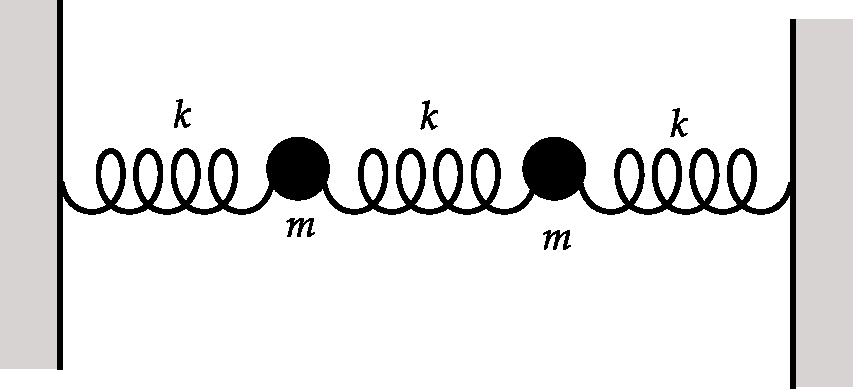
\includegraphics[height=3cm,width=5cm]{problem2}
\end{figure}
(a)Write down lagrangian of the system\\
(b)Write down equation of motion\\
(c)Write down secular equation and solve it for normal frequency.
\begin{answer}
	\begin{align*}
	&\text { (a) } L=\frac{1}{2} m \dot{x}_{1}^{2}+\frac{1}{2} m \dot{x}_{2}^{2}-\frac{1}{2} k x_{1}^{2}-\frac{1}{2} k\left(x_{2}-x_{1}\right)^{2}-\frac{1}{2} k x_{2}^{2}\\
	&\text { (b) } \frac{d}{d t}\left(\frac{\partial L}{\partial \dot{x}_{1}}\right)-\left(\frac{\partial L}{\partial x_{1}}\right)=0 \Rightarrow m \ddot{x}_{1}+k x_{1}-k\left(x_{2}-x_{1}\right)=0\\
	&\frac{d}{d t}\left(\frac{\partial L^{*}}{\partial \dot{x}_{2}}\right)-\left(\frac{\partial L}{\partial x_{2}}\right)=0 \Rightarrow m \ddot{x}_{2}+k x_{2}+k\left(x_{2}-x_{1}\right)=0 \Rightarrow m \ddot{x}_{2}+k x_{2}+k\left(x_{2}-x_{1}\right)\\
	&\text { (c) } L=\frac{1}{2} m \dot{x}_{1}^{2}+\frac{1}{2} m \dot{x}_{2}^{2}-\frac{1}{2} k x_{1}^{2}-\frac{1}{2} k\left(x_{2}-x_{1}\right)^{2}-\frac{1}{2} k x_{2}^{2}\\
	&T=\frac{1}{2} m \dot{x}_{1}^{2}+\frac{1}{2} m \dot{x}_{2}^{2}\\
	&T=\left(\begin{array}{ll}
	m & 0 \\
	0 & m
	\end{array}\right)\\
	&V=\frac{1}{2} k x_{1}^{2}+\frac{1}{2} k\left(x_{2}-x_{1}\right)^{2}+\frac{1}{2} k x_{2}^{2}\\
	&V=\frac{1}{2} k x_{1}^{2}+\frac{1}{2} k\left(x_{2}^{2}+x_{1}^{2}-2 x_{1} x_{2}\right)+\frac{1}{2} k x_{2}^{2}\\
	&V=\frac{1}{2} k x_{1}^{2}+\frac{1}{2} k\left(x_{2}^{2}+x_{1}^{2}-x_{1} x_{2}-x_{2} x_{1}\right)+\frac{1}{2} k x_{2}^{2}\\
	&=k x_{1}^{2}+k x_{2}^{2}+\frac{1}{2} k\left(-x_{1} x_{2}-x_{2} x_{1}\right)=\left(\begin{array}{cc}
	2 k & -k \\
	-k & 2 k
	\end{array}\right)\\
	&\text { The secular equation is given by }\\
	&\left[V-\omega^{2} T\right]=0, \quad\left(\begin{array}{cc}
	2 k-\omega^{2} m & -k \\
	-k & 2 k-\omega^{2} m
	\end{array}\right)=0\\
	&\left(2 k-\omega^{2} m\right)^{2}-k^{2}=0, \omega_{1}=\sqrt{\frac{k}{m}},\text{ which is normal frequency for oscillation and another value of}\\ &\omega_{2}=\sqrt{\frac{3 k}{m}} \text{which is first over-tone.}
	\end{align*}
\end{answer}
\item Two identical particle of masses m are constrained to move on a horizontal loop .Two identical spring with constant k connected the mass and wrap around the loop.If $x_1$ and $x_2$ are displacements of first mass and second mass from equilibrium point.\\
\begin{figure}[H]
	\centering
	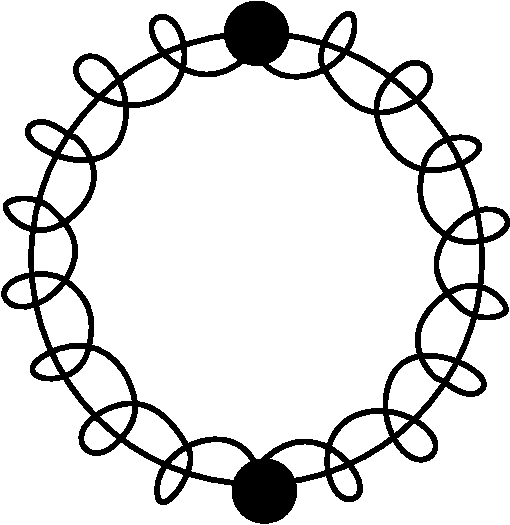
\includegraphics[height=4cm,width=5cm]{problem 3}
\end{figure}
(a)Write down lagrangian of the system \\
(b)Write down equation of motion\\
(c)Write down secular equation and solve it for normal frquency
\begin{answer}
	\begin{align*}
	&\text {(a) } l=\frac{1}{2} m x_{1}^{2}+\frac{1}{2} m \dot{x}_{2}^{2}-\left(\frac{1}{2} k\left(x_{2}-x_{1}\right)^{2}+\frac{1}{2} k\left(x_{1}-x_{2}\right)^{2}\right)\\
	&\text { (b) } \frac{d}{d t}\left(\frac{\partial L}{\partial \dot{x}_{1}}\right)-\left(\frac{\partial L}{\partial x_{1}}\right)=0 \Rightarrow m \ddot{x}_{1}+2 \dot{k}\left(x_{1}-x_{2}\right)=0\\
	&\frac{d}{d t}\left(\frac{\partial L}{\partial x_{2}}\right)-\left(\frac{\partial L}{\partial x_{2}}\right)=0 \Rightarrow m \ddot{x}_{2}+2 k\left(x_{2}-x_{1}\right)=0\\
	&\text { (c) } L=\frac{1}{2} m \dot{x}_{1}^{2}+\frac{1}{2} m \dot{x}_{2}^{2}-\left(\frac{1}{2} k\left(x_{2}-x_{1}\right)^{2}+\frac{1}{2} k\left(x_{1}-x_{2}\right)^{2}\right)\\
	&T=\frac{1}{2} m \dot{x}_{1}^{2}+\frac{1}{2} m \dot{x}_{2}^{2} \Rightarrow T=\left(\begin{array}{cc}
	m & 0 \\
	0 & m
	\end{array}\right)\\
	&I(x)=\left(\frac{1}{2} k\left(x_{2}-x_{1}\right)^{2}+\frac{1}{2} k\left(x_{1}-x_{2}\right)^{2}\right)=\frac{1}{2} k\left(2 x_{1}^{2}+2 x_{2}^{2}-4 x_{1} x_{2}\right)\\
	&V=\left(\begin{array}{cc}
	2 k & -2 k \\
	-2 k & 2 k
	\end{array}\right)\\
	&\left[V-\omega^{2} T\right]=0\\
	&\left(\begin{array}{cc}
	2 k-\omega^{2} m & -2 k \\
	-2 k & 2 k-\omega^{2} m
	\end{array}\right)=0\\
	&\left(2 k-\omega^{2} m\right)^{2}-(2 k)^{2}=0\\
	&\left(\left(2 k-\omega^{2} m\right)+2 k\right)\left(\left(2 k-\omega^{2} m\right)-2 k\right)=0\\
	&\omega=\sqrt{\frac{4 k}{m l}} \text{is normal frequency corresponding to oscillation and} \omega=0 \text{corresponding
		to translation motion.}
	\end{align*}
\end{answer}
\end{enumerate}